% !TEX root = arbeit.tex
\section{Experiments} \label{sec:Exp}
	%rewrite. Have a look how much the measurement configuration changes and state the normal measuring conditions instead of stating them always. Reference them if they do not change.
	The tests described in this chapter include tests of the different components of the NIM instrument such as laboratory tests of the flight antechamber tested on the Prototype or the flight ion-mirror. This part of Chapter \ref{sec:Exp} includes manly test with the prototype, and tests with the PFM and FS model.

	% In zeitlicher Reihenfolgen auflisten, damit man sieht, zu welchem Zeitpunkt man mit welchen Teilen gearbeitet hat.
	% In this section, all the different test (lab and simulations) are listed. As far as possible in their chronolocial order because between some lab tests there were simulations to improve the instrument before testing the redesigned instrument.

	% Fügt ein PDF ein, nummeriert nach dem PDF normal weiter.
	%\includepdf[pages=-]{Report_Thermofoil_UV_Masterarbeit.pdf}

	% Section über Detector? haben wir ja nicht wirklich etwas gemacht. Diode durch 2 Widerstände ersetzt. -> Spannungsfestigkeit. Verlauf der Überschläge. Unterschiedliche Skizzen.

	In this section, the different tests are described to develop the NIM instrument. Different parts of the instrument were tested to improve the instrument.
%-----------------------------------------------------------------------------------
	\subsection{Flight Ion-Mirror}
	% What is and ion-mirror. How does it work, compare the two designs.
	In this section the performance of the two ion-mirrors is compared. As described in chapter \ref{subsec:setupInst}, the prototype ion-mirror consists of several ring-electrodes connected with each other with resistors to generate a linear voltage gradient. The flight ion-mirror consists of a ceramic tube with two resistance spirals replacing some of the ring-electrodes. Fig.\,\ref{fig:ExpRefl} left shows the prototype ion-mirror and Fig.\,\ref{fig:ExpRefl} right shows the flight ion-mirror mounted to the NIM prototype in the test setup. An ion-mirror of the same type as the flight ion-mirror was also used in the RTOF mass spectrometer which flew in ROSINA \cite{Diss_Scherer} and the in the NGMS \cite{Diss_Hofer}. From the electrical point of view, the two ion-mirror types behave the same.\\
	\begin{figure}[h]
		\begin{subfigure}{0.5\textwidth}
			\centering
			\includegraphics[width = 0.95\textwidth]{Experiments/reflectron_Prototype1.jpg}
		\end{subfigure}
		\begin{subfigure}{0.5\textwidth}
			\centering
			\includegraphics[width = 0.85\textwidth]{Experiments/reflectron_flight.JPG}
		\end{subfigure}
		\caption{Left: Prototype ion-mirror with ring-electrodes. Right: Prototype with flight ion-mirror.}
		\label{fig:ExpRefl}
	\end{figure}
	The measurements were performed in a vacuum chamber. The residual gas pressure for the measurements with the prototype ion-mirror was 5$\cdot$10\textsuperscript{-10}mbar and for the measurements with the flight ion-mirror (PFMR) 1.4$\cdot$10\textsuperscript{-9}mbar. The test gases were injected directly through a leak valve to increase the chamber pressure up to 1$\cdot$10\textsuperscript{-8}mbar. The used test gases were: Ne, Ar, Kr and Xe. 3\, Mio. single spectra were histogramed for each of the measurements. All voltages of the instrument were optimized for the measurements with the two ion-mirrors. Table\ref{tab:refPerftab} shows the signal-to-noise ratios and the mass resolution of the different test gases measured with the two instrument configurations.\\
	\begin{table}
		\begin{center}
		\begin{tabular}{|l|r|r|r|r|}
			\hline
			Gas						&SNR ProtoR	&SNR PFMR	&m/$\Delta$m ProtoR	&m/$\Delta$m PFMR\\
			\hline
			\textsuperscript{20}Ne	&2022.9		&562.4		&200 ± 12		&236 ± 16\\
			\textsuperscript{40}Ar	&4732.6		&1808.4		&212 ±  9		&267 ± 15\\
			\textsuperscript{86}Kr	&746.1		&414.3		&224 ±  7		&292 ± 12\\
			\textsuperscript{136}Xe	&185.5		&97.1		&265 ±  8		&332 ± 13\\
			\hline
		\end{tabular}
		\end{center}
		\caption{Table listing the signal-to-noise ratios (SNR) and the mass resolution (m/$\Delta$m) of the prototype ion-mirror (ProtoR) and the flight ion-mirror (PFMR). The mass resolution in the table is underestimated to the real value.}
		\label{tab:refPerftab}
	\end{table}
	The SNR of the flight ion-mirror of the measurement with the flight ion-mirror is for all gases lower than the SNR of the measurements with the prototype ion-mirror due to the higher amount of residual in the chamber during the measurements with the flight ion-mirror. The mass resolution of all of the test gases is higher when measuring with the flight ion-mirror.
	% Only show spectrum if really required. Here it is not necessary. Only for bluffing how nice it looks like.
	
%----------------------------------------------------------------------------------
	\subsection{Flight Antechamber}
	% dimensions old antechamber: d_in = 4 mm, d_out = 3 mm, d_sp = 40 mm
	%			new:			d_in = 5 mm, d_out = 4 mm, d_sp = 80 mm
	% For further explanation of the geometry see Chap.\ref{subsubsec:Densenhan}.
	After successfully testing the flight ion-mirror, the flight antechamber was tested. A picture of the prototype and the flight antechamber is shown in Fig.\,\ref{fig:expAntchamPic}. The antechambers consist of two parts. In the old design the two parts of the antechamber had a rim on which the screws at position $\pm$45\degree were mounted to put the two parts together. Tests with this antechamber revealed that the neutral particles hit these screws and scatter into chamber (Fig.\ref{fig:AnteMeasData}a) \cite{Meyer_2017_ante}). Therefore, an antechamber with a flat outer surface was required. In the new design the screws are recessed into the 1\,\si{\milli\meter} thin surface of the antechamber to get rid of the needed rim in the old design. In addition the new antechamber is by a factor two bigger than the prototype antechamber with the aim to get more signal. Simulations of the flight trajectory revealed that two holes were required at positions $\pm$60\degree to get optimal signal \cite{SOC_Crema3p2}. The CASYMIR test facility is not able to shoot the neutral particle beam under an angle of 60\degree onto the instrument. To test the new designed antechamber, an slightly different antechamber was used with the second entrance hole at position $\theta_0 = -90\degree$ instead of -60\degree. With a rotation mechanism, the instrument can be rotated around the x-axes by $\pm$90\degree.\\
	\begin{figure}[h!]
		\begin{subfigure}{.5\textwidth}
			\centering
			\includegraphics[width=\textwidth]{Experiments/ProtoAnte.png}
		\end{subfigure}
		\begin{subfigure}{.5\textwidth}
			\centering
			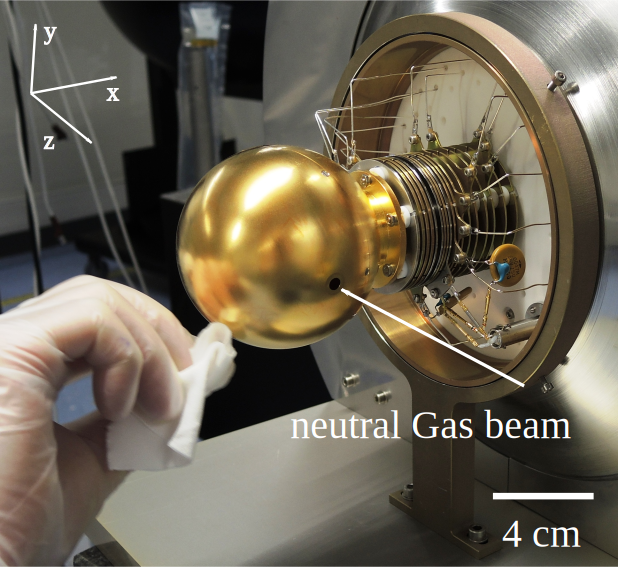
\includegraphics[width=.8\textwidth]{Experiments/FlightAnte.png}
		\end{subfigure}
		\caption{Left: Prototype antechamber. Right: flight-like antechamber with two entrance holes at positions +60\degree and -90\degree.}
		\label{fig:expAntchamPic}
	\end{figure}

	These measurements were conducted at the CASYMIR test facility at the university of Bern. CASYMIR is able to generate a neutral particle beam with velocities up to 5.5\,\si{\kilo\meter\per\second} \cite{CASYMIR_Graf2004}. For these measurements the particle velocity was about 2.5\,\si{\kilo\meter\per\second} because this is the velocity of the spacecraft in Ganymede orbit, which will be 90\% of the measuring time of NIM.\\
	\begin{figure}[h!]
		\begin{subfigure}[t]{.5\textwidth}
			\centering
			\includegraphics[width=\textwidth]{Experiments/oldAnte_ThMode.png}
			\caption{Old antechamber, thermal mode.}
		\end{subfigure}
		\begin{subfigure}[t]{.5\textwidth}
			\centering
			\includegraphics[width=\textwidth]{Experiments/oldAnte_NMode.png}
			\caption{Old antechamber, neutral mode.}
		\end{subfigure}
		\begin{subfigure}[b]{.5\textwidth}
			\centering
			\includegraphics[width=\textwidth]{Experiments/newAnte_ThMode.png}
			\caption{New antechamber, thermal mode.}
		\end{subfigure}
		\begin{subfigure}[b]{.5\textwidth}
			\centering
			\includegraphics[width=\textwidth]{Experiments/newAnte_NMode.png}
			\caption{New antechamber, neutral mode.}
		\end{subfigure}
		\caption{Panel a) an b) show measurements done with NIM Prototype sensor with the old antechamber attached. a) shows measurement conducted with the thermal gas mode and measurement of panel b) were conducted in neutral mode respectively \cite{Meyer_2017_ante}. c) and d) are the same corresponding measurements but performed with the new antechamber attached to the NIM instrument.}
		\label{fig:AnteMeasData}
	\end{figure}

	Fig.\,\ref{fig:AnteMeasData}~a) shows measurements conducted with the thermal mode when the old antechamber was attached \cite{Meyer_2017_ante}. For these measurements, the instrument was rotated around the x-axis by keeping the beam at the same position. When rotating the antechamber, the hole moves out the neutral particle beam because the beam is smaller than the antechamber. The expected intensity $I_{ant}$ is the result of the function of the moving hole through the beam with a normal distribution:
	\begin{equation}
		I_{ant} = \frac{A}{\sigma\sqrt{2\pi}}\int_{x_{min}}^{x_{max}} \exp^{\frac{(x-\mu)^2}{2\sigma^2}} dx
	\end{equation}
	With $A$ a constant taking the beam intensity into account, $\sigma$ the standard deviation of the beam and $\mu$ the position of the beam centre relative to the centre of the antechamber which is equal 0. The borders of the integral determine the part of the beam entering the antechamber:
	\begin{align}
		x_{max} &= r_{ant}\sin{\alpha} - r_{aHi}\cos{\alpha}\label{eq:antIntgrLimHigh}\\
		x_{min} &= r_{ant}\sin{\alpha} + r_{aHi}\cos{\alpha}\label{eq:antIntgrLimLow}
	\end{align}
	With $r_{ant}$ the radius of the antechamber and $r_{aHi}$ the radius of the antechamber entrance hole. The sine contribution considers the shift of the hole in y-direction when the hole is rotated. The cosine contribution comes from the projection of the beam on the entrance hole. For the measurements with the new antechamber, the shift in y-direction when rotating the instrument was compensated by shifting the whole instrument. Therefore the sine contribution in Eq.\eqref{eq:antIntgrLimHigh} and Eq.\eqref{eq:antIntgrLimLow} cancels out leading to a more cosine-like function.\\
	When comparing Fig.\,\ref{fig:AnteMeasData}~a) and b), we see that with the new design we successfully got rid of the artefacts previously induced by the mounting screws of the old design. The higher intensity at angle +90\degree is most probable an outlier because it appears in both the thermal (Fig.\,\ref{fig:AnteMeasData}~b)) and the neutral mode graphic (Fig.\,\ref{fig:AnteMeasData}~d)) of the measurements with the new antechamber. The drop in signal intensity when measuring with the thermal mode channel compared to the old measurements is a result of having two an additional entrance hole which was necessary because of the flyby trajectories (see Chap.\ref{subsubsec:Densenhan}).\\	
	Fig.\ref{fig:AnteMeasData}~b) shows measurements conducted with the neutral gas mode with the old antechamber attached and Fig.\ref{fig:AnteMeasData}~d) shows measurements conducted with the neutral gas mode when the new antechamber was attached. At position $\pm$30\degree and $\pm$90\degree there are pillars holding the stack of the ion-optical lenses together. When the beam hits these pillars, the particles scatter in all directions leading to a damping of the signal. For the neutral gas channel, no difference in the signal distribution is expected because a change in the antechamber design does not influence the signal measured with the neutral gas channel. At 0\degree the signal is significantly higher than on the other plateaus. When shooting under this angle into the source, the neutral particle beam is in line with the electron beam leading to a higher signal. Another explanation is, that a different voltage set for the voltages in the ionization region changes the distribution of the electron beam thus leading to a different ion distribution in the ionization region. This leads to a different angular distribution of the signal for the neutral gas channel when comparing the results of the two measurement series. The difference in signal intensity also comes from the better voltage set. Some times its just enough to tune on the right electrode to get a signal amplification of a factor 2.\notes{rewrite that explanation.}
	
	% Picture of that simulation. Only ions produced over the central grid reach the detector. \\titania.unibe.ch\UserHomes\foehn\My Documents\PhD\Presentations\PEP_CASYMIRD_data_180531.pptx
	
%-------------------------------------------------------------------------------------	
	\subsection{Entrance characterization}
	\notes{rewrite title.}	
	
	\begin{figure}[h!]
		\centering
		\includegraphics[width=\textwidth]{Experiments/2D_scan_anteEntr.jpg}
		\caption{Left:Intensity profile when shooting with the neutral particle beam at the structure of the NIM PFM instrument. Right: Front view as seen by the neutral particle beam.}
		\label{exp:PFMIntCharTot}
	\end{figure}
	\begin{figure}[h!]
		\centering
		\includegraphics[width=.7\textwidth]{Experiments/2D_scan_Ant.png}
		\caption{Zoom on the antechamber hole when shooting with the neutral particle beam at the structure of the NIM PFM instrument.}
		\label{exp:PFMIntCharAnt}
	\end{figure}	
	\begin{figure}[h!]
		\centering
		\includegraphics[width=\textwidth]{Experiments/2D_scan_Entr.jpg}
		\caption{Zoom on the entrance when shooting with the neutral particle beam at the structure of the NIM PFM instrument.}
		\label{exp:PFMIntCharEnt}
	\end{figure}	
	For the first tests with the NIM PFM, the front side of the NIM instrument was scanned with the neutral particle beam to find the position of the entrance slit and the antechamber entrance hole to align the beam properly with the instrument. Fig.\,\ref{exp:PFMIntCharTot} left shows the scan of the front side and the right picture shows the corresponding structural part. The hole of the antechamber is clearly visible as a small dot. Fig.\,\ref{exp:PFMIntCharAnt} shows a zoom with a better resolution of the antechamber entrance hole which shows a nice Gaussian distribution as expected. When looking at the entrance slit, there are two positions with increased intensities. The zoom on Fig.\,\ref{exp:PFMIntCharEnt} reveals that the positions of biggest intensity is were the beam hits the structure covering the two electron emitting filaments. The other intensity maximum is where the beam hits the supporting structure opposite of the filament bloc. When the gas hits these structures, the gas slows down leading to a local increase of the gas density. Therefore, the structure partially thermalizes the gas similar as the closed source antechamber. This was not intended because with the neutral gas channel the aim is to measure incoming particles directly without any interaction with the structure. In the design of thE PFM, the filament bloc and the supporting structure act like a funnel directing the sputtered gas to the central grid. The intensity amplification when shooting on the filament bloc is unavoidable. For the supporting structure opposite of the filament, a pillar instead of the plate like structure would have been the better option. When the gas hits the pillar, the pillar scatters the gas in all direction instead of scattering only in the direction of the central grid. This phenomenon was observed when doing a similar measurement with the NIM prototype (Fig.\,\ref{exp:ProtoIntCharEnt}).\\
	The ion-source of the prototype had six pillars holding the different focusing lenses together. In Fig.\,\ref{exp:ProtoIntCharEnt} the pillars are marked as red circles. The prototype had also an electron emitting filament. For these measurements, the ionization region was scanned with the neutral particle beam at angles 0\degree and $\pm$60\degree to shoot between the pillars. When scanning from the front side, the signal intensity has a nice Gaussian shape. When shooting at angles of $\pm$60\degree the Gaussian distribution is visible when the neutral particle beam is aligned over the centre grid with an asymmetry toward the side of the filament. The filament bloc slows down the neutral particles leading to a small amplification of the signal. This amplification is less dominant than in the design of the PFM because the part of the filament structure seen by the beam is tilted outward. At distances bigger than $\pm$25\,mm from the centre, the signal drops again. This is where the beam is completely outside of the ionization region.
	\begin{figure}[h!]
		\centering
		\includegraphics[width=\textwidth]{Experiments/Entrence_Proto_topview.png}
		\caption{Zoom on the entrance when shooting with the neutral particle beam at the structure of the NIM Prototype. The red circles mark the positions of the pillars holding the ion source together.}
		\label{exp:ProtoIntCharEnt}
	\end{figure}
	
%--------------------------------------------------------------------------------------------	
	\subsection{Shutter Performance Test}
	When measuring with the neutral gas channel, the aim is that the particles are measured directly without any interaction with the structure of the instrument. Therefore, a shutter between the antechamber and the ionization region was required to close the particle entrance from the antechamber. In this section the performance of the shutter was tested. According to the model stated in Chap.\ref{subsubsec:motorflow} the shutter should damp the signal by a factor 600.\\
	These tests were performed with the NIM PFM \notes{Ref. as soon as the two models are properly described in the Setup section.}. The PFM was operated with laboratory electronics. The tests were performed at the CASYMIR test facility. The used particle beam consisted of hydrogen and xenon with a velocity of 2\,\si{\kilo\meter\per\second}. Three different measurements were performed: One with the beam directing onto the antechamber with the shutter open, one with the shutter closed and a background measurement, where the particle beam was pointed onto the outer structure of NIM to estimate how much of the signal arises from the test gas scattering into the ionization region when the beam is directed in an arbitrary direction. This background was subtracted from both signals before they were divided through each other to determine the damping factor $G_{close}$ of the shutter.\\
	The damping factor of the shutter according to the measurements is 12 instead of the required 1000. The biggest impact has the actual thickness of the gap between the shutter and the antechamber when the shutter is closed. The damping reduces significantly when the gap is bigger than actually designed. This is shown in Fig.\,\ref{fig:ShutGapSizeSigDamp} in Chap.\,\ref{subsubsec:motorflow}. With a gap size of about 0.1\,mm instead of 0.01\,mm the damping factor is only about a factor 25. Other reasons are that the portion of the beam which scatters on the antechamber outer walls gets thermalized in the vacuum chamber and adds to the signal intensity. In the outer space, the gas scatters on the antechamber but does not reach the ionization region because it will flow around the instrument.
	
	\begin{comment}	
	\begin{table}
		\begin{center}
			\begin{tabular}{|c|c|c|}
				\hline
				\multirow{2}{*}{Configuration} & \multicolumn{2}{c|}{Species Area [a.u.]} \\
				\cline{2-3}
				& \textsuperscript{129}Xe & \textsuperscript{132}Xe \\ \hline
				Shutter open  & 36.97 ±0.07 & 36.7 ±0.06\\
				Shutter close &	6.76 ±0.07 & 6.7 ±0.05\\
				Background & 3.87 ±0.05 & 3.73 ±0.03 \\
				\hline
			\end{tabular}
		\end{center}
		\caption{The signal intensity is given for different shutter positions. It is proportional to the number of measured particles. The background was determined by shooting with the beam onto the outer structure of NIM.}
%		\label{tab:measShutMot}
	\end{table}
		% IsoArea [10^9]
		
	\begin{table}
		\begin{center}
			\begin{tabular}{|c|c|c|c|c|}
				\hline
				\multirow{2}{*}{Configuration} & \multicolumn{4}{c|}{Species Area [a.u.]} \\
				\cline{2-5}
				&N\textsubscript{2}& CO\textsubscript{2} & \textsuperscript{129}Xe & \textsuperscript{132}Xe \\ \hline
				Shutter open & 18.36 ±0.07 & 10.76 ±0.06 & 36.97 ±0.07 & 36.7 ±0.06\\
				Shutter close & 19.57 ±0.07 & 12.04 ±0.06 &	6.76 ±0.07 & 6.7 ±0.05\\
				Background & 18.43 ±0.07 & 11 ±0.06 & 3.87 ±0.05 & 3.73 ±0.03 \\
				\hline
			\end{tabular}
		\end{center}
		\caption{The signal intensity is given for different shutter positions. It is proportional to the number of measured particles. The background was determined by shooting with the beam onto the outer structure of NIM. N\textsubscript{2} and CO\textsubscript{2} are part of the residual gas and Xe is the test gas in the neutral particle beam.}
%		\label{tab:measShutMot}
	\end{table}
	
	\begin{table}
	\begin{center}
		\begin{tabular}{|c|c|c|c|c|c|c|c|c|}
			\hline
			\multirow{2}{*}{Configuration} & \multicolumn{4}{c|}{m/$\Delta$m}& \multicolumn{4}{c|}{SNR} \\
			\cline{2-9}
			&N\textsubscript{2}& CO\textsubscript{2} & \textsuperscript{129}Xe & \textsuperscript{132}Xe & N\textsubscript{2} & CO\textsubscript{2} &\textsuperscript{129}Xe&\textsuperscript{132}Xe\\ \hline
			Shutter open & 307$\pm$25& 330$\pm$23 & 361$\pm$16& 373$\pm$17 & 550.8 & 309.9 & 735.7 & 740.2\\
			Shutter close &307$\pm$25& 330$\pm$23 & 361$\pm$16& 365$\pm$16 & 540.3 & 315.4 & 120.8 & 121.6\\
			Background &307$\pm$25& 330$\pm$23 & 353$\pm$15& 357$\pm$16 & 631.6 & 360.2 & 85.4 & 84\\
			\hline
		\end{tabular}
	\end{center}
	\caption{Mass resolution m/$\Delta$m and Signal-to-Noise Ratio for different shutter positions. N\textsubscript{2} and CO\textsubscript{2} are part of the residual gas and Xe is the test gas in the neutral particle beam.}
%	\label{tab:measShutMot}
	\end{table}
	
	\end{comment}	
	

	
%--------------------------------------------------------------------------------
	\subsection{Simulations}
	
	During development, the mounting of the HV lenses was adapted. Simulations had to be done because as a result of the changed form of the lenses, the voltage set also changed. In this case, the voltage ranges increase by about blabla volts. These new higher ranges challenged the design of the supply electronics because the electronics has a limited amount of space. % Look up the details. Explanation with the electric fields?
	
	%\textcolor{red}{\textbf{Simulations of the adaption of the mounting of the electrodes has to come before the experiments with the PFM although the PFM structure is explained before.}}
	
	% Maybe an other arrangement of the Simulations chaper. See whicht simulations are performed how far any in which order they have to be to be comprehendible.
	
	% Evt. in einem eigenen Kapitel? Schauen, welchen Einfluss es dann jeweis auf die Hardware hatte. -> Elektronik setzt Spannungsranges, beschreiben, dass man da iterieren musste um das optimale Simulationsspannungsset zu finden mit den Grenzen, welche die Elektronik uns für die jeweiligen Elektroden gibt. -> vgl. mit den Messungen vom PFM.
	% Neusimulationen mit neuen Grenzen für die HV. -> die Resultate dieser Simulationen. Als Folgen davon wurden die Grenzen für die HV neu definiert. Schauen, wie man das am besten auseinander nimmt :/.

	% Change of the mounting of the IS lenses -> change in voltages

	% Pulsersimulationen -> Kriterien für Andy für das Pulserdesign. Ab wann wir einen Einbruch in der Massenauflösung haben. (Worddokument wo die einzelnen Bilder zusammengestellt sind?)
	
	% Filament repeller simulation tests. Noch Graphiken einmal einfügen. Die wichtigsten.
	% Um herauszufinden, wie wichtig die Position des Filaments ist.
	
	% Noch besser umschreiben. Die position des filaments entspricht nicht der erwarteten??? Was ist da schief gelaufen??? :(
	
	% Intensitätssimulation Countberechnung:
	% Man generiert 2000 e- auf dem Filament und zeichnet immer nach 1E-5 microsec auf, an welcher Position sich die Teilchen gerade befinden. Die Fkt. 'Plot_optVoltAndPos.m' zählt alle Positionen zusammen, welche sich in dem Zylindervolumen befinden. Die Grundfläche des Zylinders ist das Eintritts-Grid von der antechamber und die Höhe ist die Höhe der Entrance. Im th-Mode befinden sich nur in diesem Volumen neutrale Teilchen.
	\begin{figure}[h]
		\begin{subfigure}{0.53\textwidth}
			\centering
			\includegraphics[width= 0.95\textwidth]{Experiments/SimRepPosU.png}
		\end{subfigure}
		\begin{subfigure}{0.47\textwidth}
			\centering
			\includegraphics[width= 0.95\textwidth]{Experiments/SimRepPosImax.png}
		\end{subfigure} %0.95
		\caption{Left: The filament repeller voltage to reach the maximum electron intensity over the volume of the neutral particles. Right: Electron intensity normed on the intensity at position 0.} % Noch Graphik wie Intensität bei den versch. Pos abfällt.
		\label{fig:ExpSimRep}
	\end{figure}

	\subsection{Filament decision}
	% Ranking criterion -> Explanation, see electronics book. constant power of one filament -> resistance variies over time. Vgl. Diss Rico.

%------------------------------------------------------------------------------------
	\subsection{Pulser}
	% high mass have better mass resolution than low masses -> ok except that N2 (28 u) and H2O(18u) have a similar mass resolution.
	% Impact of the falling edge of the pulser should be better visible. With increasing pulse voltage, the fall time increases and the mass resolution drops. Is barely visible and within the calculated errorbar. No clear statement for the verification can be made. For the higer mass particles the tendency is surprisingly better visible. Is it also related to the applied HV?
	
	% The focusing of the HV lenses has a bigger impact on the heavy species than on the light ones.
	% Mass resolution of the light species depends on the fall time. When the fall time is short enough, all particles get the same amount of energy.


	% Best value for the pulser high voltage also depends on the rest of the voltage set. Assume that the voltage set is optimized for the different values... it is easier to focuse slow particles... that depends on the pulser as it is shown in Davides Paper.
	
	% source thickness
	% slit thickness of 2mm and m = 1u -> 3ns to leave the source
	%							m = 2u -> 4.5ns H2
	%							m = 10u -> 10ns
	%							m = 100u -> 32ns
	%							m = 130u -> 37ns
	
	% Simluations of the required pulser shape were performend by Stefan Meyer. They should be documented in his simulation lab book. The outcome was the shape in his Diss.
	% How much conpensate the effect of the different spacial distribution the rise time?
	% We do not have the stability of the baseline of the high voltage pulse and the stability at the high plateau. So we cannot analyse and discuss that with these measurements.



	
	% Simulations with different rise times and their influence on the mass spectrum. Look at the data available. Just shows that the rise time has no big impact. Results also from the calculation. Are there other more important properties?
	% Test with lab pulser, wavelab pulser -> compare their properties and their performance.
	
	% Pulsertests, Messungen, Simulationsresultate. Write something and discuss it with Peter.
	% Two different pulsers properties, pulse shape. Tests with different gases. Massresolution, Intensity relation?, SNR? Are these two properties correlated? Noch mit Peter anschauen.
	
	
	% Messungen
	% \\titania.unibe.ch\UserHomes\foehn\My Documents\PhD\Messungen\PFM\PFM_1905to1911\PulserTests_191015_to_17
	% \\titania.unibe.ch\UserHomes\foehn\My Documents\PhD\Simulations\Pulser_risetime_and_HV_sim
	% settings
	% \\titania.unibe.ch\UserHomes\foehn\My Documents\PhD\NIM
	% Look at the data for the slow species such as H2, H2O,.. thus the falls time is more crucial for the slow species.
	
%----------------------------------------------------------------------------------------------	
	\subsection{Detector Tests}
	% Put the Calibration and discussion of Ustack vs. UMCP in that Chapter. It can later on still be moved into the Setup chapter. Show the fit parameter for the curve for calibration purpose.
	% Discussion about upper part of the curve. Discuss that with the plot showing the differences to the model if there is a logical explanation. May discuss that again with Peter. Which possibilities thereare.
	
	\begin{figure}[h]
		\centering
		\includegraphics[width=.7\textwidth]{Experiments/PFM_UstackUmccp_TimeEvol.png}
		\caption{Dependence of the MCP voltage (U\textsubscript{MCP}) from the voltage applied over the detector (U\textsubscript{stack})}
		\label{fig:PFMUstackUmcpTimeEvol}
	\end{figure}
	% fit parameters: ax +b; a = 0.932, b = 12 V
	
	% FS IsoArea. Variation of the MCP gain an observation how the SNR and IsoArea change. \\titania.unibe.ch\UserHomes\foehn\MyDocuments\PhD\Messungen\FS\ firstOpti\MCP_Gain.opj
	% Also show different signal heights/ forms? Defect diode, functioning diode (not available), resistor? Full gain curve is only possible for functioning diode (tests to be done (no data available)) and resistor (plot already included).
	The following chapter describes improvements of the mechanical and electrical design of the NIM PFM detector and tests performed with different versions. Most of the tests were performed in the Pumpstand nr.2 (Chapter \ref{subsubsec:SetFacPumpst}) and a few were done with the detector in the sensor Proto Flight Model (PFM) or in the sensor flight spare model (FS).\\
	% Leave this part here as it is a description of the process we were working on. Describe the adaption of the meachanical design of the detector housing, the consequence that we inserted a resistor instead of an anode. Pros and Cons of the Anode vs. the resistor?
	% Description of the housing and problems related to it -> investigation, improvements.
	
	% Explanation of the discharge problem and the redesign of the detector housing. Several figures and graphics are missing at that 
	
	The detector suffered repeatedly discharges causing a failure of the diode, which is one of the key components of the detector. This lead to a redesign of the detector housing and to an exchange of the diode through a resistor, because the resistor is more robust concerning discharges. % Include an electrical schema. May a zoom of the other one laready included in the setup chapter (as soon as it is finished). Explanation about how a diode works? Talk with JoGa maybe. Explain main hypothesis why it died repeatedly?
	The discharges could be eliminated by a redesign of the detector housing. % Vgl. Fig. of the 2 housing designs (start and end) and explain them.
	Fig.bla left shows an earlier version of the detector housing and Fig. bla right shows the design of the current flight detector.
	Basically, the MCPs lay on a border about 1 mm above the anode. % Check distance
	A diode generates an additional voltage difference between the MCP backside and the anode to accelerate the electrons from the MCP backside towards the anode. Between this border and the MCP is the contact lug which is connected to the high voltage rail. On top of the upper MCP is the contact lug to connected to the corresponding voltage rail. On top of that is a bushing and a sort of screw. When tightening the screw, the bushing presses uniformly on the MCPs. In the old design, the thread for the screw was cut down to the boarder on which the MCPs lay. When assembling the whole stack, the MCPs often cant in the thread. Another challenge lay in tightening of the screw. When the screw was too loose, the top and the bottom contact lug had no reliable contact to the MCPs. When applying a high voltage over the whole MCP stack, the gap acts as an additional resistor over which the voltage build up resulting in a discharge between the corresponding electrode and the MCP. The discharge can propagate through the whole MCP stack and damage the diode and the capacitors. When the screw was tighten too much, the MCPs broke as they consist of lead glass and are very delicate in the mechanical point of view. As a consequence, the screw thread was cut less deep down and an additional boarder was made on which the bushing was pressed by the screw to make the assembly of the detector easier. In addition, the diode was exchanged through a resistor because the resistor is more robust in regards to the discharges. Due to the uncertainty in the manufacturing process of the detector housing, spacer rings are added between the bushing and the MCP to really close the gap. Due to that uncertainty, the number of rings needed for each detector has to be determined by trial.
	% Insert a Figure of the housing. Further explanation of the design
	% free play = thechnisch für Spiel
	% Circuit diagram with both options diode and resistor. Ref for that statement?
	% Upgrade SNp6.
	
	% Explanation of the different meas Figs.
	% Detector with broken anode is detector EM4. Look if there are any specifications. Seems to have most probable the same configuration as the other detectors. -> Sufficient for the data analysis but it would be good to have the datasheet.
	Fig. \notes{bla} shows the signal shapes of different detector configurations beginning with the shape of a detector with a broken diode. The other two figures show the signal shape of a detector with a functioning diode and a functioning resistor. The most remarkable feature is that the signal height of the detector is much smaller and much broader that the signal shape of the other two configurations. In addition, the first overshoot is much lager due to the impedance mismatch caused by the broken diode. A broken diode gets conductive and therefore the potential at the MCP backside is equal to the potential of the anode. The electrons are not additionally accelerated and therefore the resulting signal is smaller than the signal with a functioning diode.\\
	Fig.\ref{fig:SN4p54p7Gain} shows the gain curves of two potential FS detectors both in the configuration with a 10\,\si{\mega\ohm} resistor instead of a diode. 
	% Other parameters to analyse? Pulse width of the 3 configurations? Overshoot? Can that really be calculated out of the data? Impedance match based on the overshoot.
	\begin{figure}[h]
		\begin{subfigure}{.5\textwidth}
			\centering
			\includegraphics[width=0.9\textwidth]{Bilder/Gain_Curves_SN4p5_4p7.png}
		\end{subfigure}
		\begin{subfigure}{.5\textwidth}
			\centering
			\includegraphics[width=0.9\textwidth]{Bilder/SN4p7_discharge.png}
		\end{subfigure}
		\caption{Left: Gain curves of two NIM PFM detectors. The difference in gain is because for each measurement curve, a different set of MCPs was used. Right: Gain curves of a folded NIM PFM detector. The lower gain curve was recorded after a discharge at an MCP voltage of 1.8\si{\kilo\volt}.}
		\label{fig:SN4p54p7Gain}
	\end{figure}
	% Discussion about the discharge behaviour in regards to gain. Are there any values? Something with free electrons destroying the inner coating of the MCP channels. Only a rough estimate needed.
	% Explanation of the fit model in theory part. -> Maike if there is any theory about that topic specifically.	
	
	% ROSETTA? When was a resistor latest used? Have a look if there is a space for sort of improvements of the sensor. If it is part of the experiments of of the thery part...
	% Explain, which measurements were made with which MCPs, describe how the discharge influences the signal. How much of the signal we loose in this specific measurement. Literature references?
	% Description of the current measurement of the detector with the laboratory electronics attached and then the calculation of the MCP voltage. State clearly under with circumstances the calculation with this method is possible and under which it is not (ion current, which is falsely taken into account)
	% Precise can we estimate the numbr of ions/ the partial pressure of the gas?
	% Describe, how far we tried to approximate the voltage.
	
	% Plot off the gain curves of the detector in its different states. flat, folded, folded in the wolfram copper shealding.
	% Measuring settings. Turn the drift voltage up to -2.5 kV and then slowly increase the anode voltage to the value you want to measure. The gain is calculated with the software by doing a Simpson 3/8 integration of the peak = Q. (Look in the lab book for the proper calculation)
	% Maybe there is time to redo the tests with the real PFM detector (XD wär schön. Leider nein). (Die Resultate sind nicht so vollständig wie die von der einen anderen Messung. Messung mit einem Zwillingsdetektor und von diesem auf den Flugdetektor schliessen. -> evt. schöne Graphik).
	
	
%-----------------------------------------------------------------------------------
	\subsection{Ionoptics}
	\subsubsection{Voltage Optimisation}
	Two types of electrical lenses. positive and negative voltage lenses. positive and negative voltage lenses have the same effect. In negative voltage lenses, the particles fly faster = shorter time-of-flight. This results in a better mass resolution.\\
	Aim in the lab is to get two different voltage sets. One for positive voltages to not stress the equipment and one with negative voltage lenses to reach the maximal performance of the instrument. -> Tests showed no significant better mass resolution. A more detailed data analysis has to be made. % data in folder: \\titania\UserHomes\foehn\My Documents\PhD\Messungen\PFM\CASYMIR-C\nMode_voltageSet_Comparison_200430 
	
	
	
%---------------------------------------------------------------------------------------------	
	\subsection{Instrument performance tests}
		% At the end, make a comparison of the discussion of the different instruments as mass resolution, SNR as far as possible.
		\subsubsection{Prototype} % Final results. Only shpw best mass resolution achieved. May revere to Stefan's Diss. With the Prototype there were mainly componenets tests.
		\subsubsection{PFM} % Include here the paper because it gives a very good overview over the results conducted with it.
		\subsubsection{FS} % Include here the final results of the FS of this year with lab and flight electronics. Discussion about that subject, see PFM paper.
		% Laboratory and flight electronics are part of the same chapter because with the fligh electronics the only thing worth to discuss is the mass resolution because the signal intensity is still very low. Discuss the SNR graphics with Peter and then finalize this part of the chapter.
		
		% Look up the conditions for the description.
		\textbf{Ion Storage two different velocities}\\ % Ref. to Abplanalp paper.
		Ion storage is very crucial for a time of flight mass spectrometer because every ion generated and not stored in the ion source is lost and can generate additional electrical noise on the detector signal line. In this test the ion storage behaviour of the ion source was analysed for thermal and neutral mode for hydrogen and krypton with velocities of 2\,\si{\kilo\meter\per\second} and 4\,\si{\kilo\meter\per\second}. The emission current was varied from 20 to 600\,\si{\micro\ampere}. Ion storage of positive ions in x- and y- direction is supported by the negative potential generated by the electron beam. Two ring electrodes with a positive voltage applied generate a positive potential ring to trap generated ions in y- and z- direction (Fig.\ref{fig:ExpFSFlightSenIonStorIS}). For emission currents from 20 to 600\,\si{\micro\ampere} according to Eq.\,\eqref{eq:elPotIem} the negative potential in the centre of the electron beam is -0.08-(-2.59)\,\si{\volt}. Fig.\ref{fig:ExpFSFlightSenIonStor} left shows the ion storage behaviour of the ion source of hydrogen and right the ion storage behaviour of krypton. In case of no ion storage, the relationship between the electron emission current I\textsubscript{em} and the signal intensity is linear. In case of ion storage there is a quadratic relationship between I\textsubscript{em} and the signal intensity. When measuring with the thermal mode, the particles get slowed down until they have energies in the range of 0.01\,\si{\electronvolt} and are therefore easy to trap in the potential field. In neutral mode particles enter the ionisation region directly. The kinetic energy of hydrogen for velocities between 2-4\,\si{\kilo\metre\per\sec} is 0.07-0.27\,\si{\electronvolt}. It can therefore easy be trapped in the potential field by the electron beam and the potential of the ring electrode already with very emission currents as low as 20\,\si{\micro\ampere}.\\
		The kinetic energy of \textsuperscript{84}Kr for the same velocities is 2.8-11.2\,\si{\electronvolt}. This energy exceeds the potential of the centre of the electron beam and the ions are therefore more difficult to trap with only the electron beam. The ions are kept in the middle of the ionisation region with the positive potential ring. According to Fig.\,\ref{fig:ExpFSFlightSenIonStor} ion storage for \textsuperscript{84}Kr starts to dominate at emission currents of 100\,\si{\micro\ampere}.
		%Therefore there is no difference in the measured intensities for hydrogen when it enters with 2 or 4\,\si{\kilo\meter\per\second}.\\		
		In thermal mode, an increase in beam velocity leads to an increase in signal intensity due to the density enhancement effect \textcolor{red}{(Ref.)}. Therefore a higher signal intensity is expected in thermal mode for 4\,\si{\kilo\meter\per\second} compared to 2\,\si{\kilo\meter\per\second}. 
		Like the in PFM, the FS shows a nice ion storage behaviour. For krypton ion storage just starts at an emission current of 100\,\si{\micro\ampere} where hydrogen is stored already at lower emission currents due its lower kinetic energy at the same beam velocity.
		
		\begin{figure}[h]
			\centering
			\includegraphics[width = 0.8\textwidth]{Experiments/FiL_IS_elBeam_Storage.png}
			\caption{Ion storage source with sample voltage set applied to the electrodes. In light blue are the potential lines and in dark blue a simulated electron beam.}
			\label{fig:ExpFSFlightSenIonStorIS}
		\end{figure}
		
		
		\begin{figure}[h] % Ion storage. Exchange Graphics as soon as discussed with Peter how to proper show the results.
			\begin{subfigure}{0.5\textwidth}
				\centering
				\includegraphics[width = \textwidth]{Experiments/FSLabIonStorageH2.png}
			\end{subfigure}
			\begin{subfigure}{0.5\textwidth}
				\centering
				\includegraphics[width = \textwidth]{Experiments/FSLabIonStorageKr84.png}
			\end{subfigure}
			\caption{Ion storage measurement with the flight spare sensor but with laboratory electronics attached for H$_2$ and $^{84}$Kr for two different gas velocities.}
			\label{fig:ExpFSFlightSenIonStor}
		\end{figure}

		% Detector behaviour test in FS sensor. Formula derivation is in the theory part with the proper detrivation.
		% No saturation observed. 

		\textbf{Mass resolution and Signal-to-Noise Ratio}\\
		According to the requirements stated in (Ref.) % See paper
		the required mass resolution for neutral mode is 500 and for thermal mode it is 1000 m/dm but to be able to distinguish between different masses at unit masses of 1000\,u NIM has to have a mass resolution of 1000. Otherwise NIM the different unit masses cannot be distinguished. Fig.\,\ref{fig:ExpFSFlightSenMassRes} show two spectra recorded with the NIM flight sensor with laboratory electronics attached with an electron emission current of 100\,\si{\micro\ampere}. With a mass resolution of 708 for neutral gas mode NIM fulfils the requirements. In thermal gas mode the highest mass resolution achieved was 830 m/$\Delta$m which comes close to the requirements. Fig.\,\ref{fig:ExpFSFlightElMassRes} show the mass spectra recorded with the NIM flight sensor with the flight electronics attached. The electron emission current was 200\,\si{\micro\ampere} the highest mass resolution achieved at the current state is 490 m/$\Delta$m for neutral gas mode and 462 m/$\Delta$m for thermal mode. Fig.\,\ref{fig:ExpFSFlightElK78} shows a mass spectrum recorded in thermal mode with an emission current of 300\,\si{\micro\ampere} the $^{78}$Kr peak is clearly visible. The signal to noise ratio for the spectra recorded with the flight electronics is very low compared to the SNR for the spectra recorded with the laboratory electronics. We also observe noisy part wandering between the single spectra. There is a significant part of repetitive noise appearing not always at the same position in the spectrum. With a proper noise filter this noise can be detected and significantly reduced without affecting the mass signal peaks. For future work, there is a lot of potential for improving the spectrum by proper analysing the noise and writing filters to suppress the noise.\\
		Fig.\,\ref{fig:ExpFSFlightSenSNR} shows a mass spectrum recorded with the flight sensor with the laboratory electronics attached. The highest SNR achieved was $6\cdot10^{5}$ and therefore almost 6 decades. % Explanation why the 6 decades are required.
		The mass peaks 355\,u, 390\,u and 429\,u are some oil components with water adducts coming from the used turbo pumps of the test facility. 415\,u is an artefact coming from the background subtraction algorithm. The artefact peak is also wider then the other surrounding mass peaks.
		
		\begin{figure}[h]
			\begin{subfigure}{0.5\textwidth}
				\centering
				\includegraphics[width = \textwidth]{Experiments/FSLabthMode.png}
			\end{subfigure}
			\begin{subfigure}{0.5\textwidth}
				\centering
				\includegraphics[width = \textwidth]{Experiments/FSLabnMode.png}
			\end{subfigure}
			\caption{Mass spectra measured with the flight spare sensor with the laboratory electronics electronics attached. Left: with thermal gas mode Right: neutral mode.}
			\label{fig:ExpFSFlightSenMassRes}
		\end{figure}

		% Mark the noisy part for better description to explain that
		% conditions: nMode UMCP: 1950 V. P = 1.03e-8 mbar 20H2:1Kr
		%			thMode UMCP = 1950 V. P = 6.05e-8 mbar
		\begin{figure}[h]
			\begin{subfigure}{0.5\textwidth}
				\centering
				\includegraphics[width = \textwidth]{Experiments/FSthMode200uA.png}
			\end{subfigure}
			\begin{subfigure}{0.5\textwidth}
				\centering
				\includegraphics[width = \textwidth]{Experiments/FSnMode200uA.png}
			\end{subfigure}
			\caption{Mass spectra measured with the flight spare instrument with the flight electronics attached. Filament emission current was 200 \si{\micro\ampere}. Left: with thermal gas mode Right: neutral mode.}
			\label{fig:ExpFSFlightElMassRes}
		\end{figure}
		
		\begin{figure} % Point out at that picture that the Kr 78 isotope is clearly visible.
			\centering
			\includegraphics[width = 0.6\textwidth]{Experiments/FS_thMode300uA.png}
			\caption{Mass spectra measured with the flight spare instrument with the flight electronics attached. Filament emission current was 300 \si{\micro\ampere}.}
			\label{fig:ExpFSFlightElK78}
		\end{figure}
		
		% SNR 600 uA emission current. Rest gas Ptot = 1.6e-9 mbar, UMCPeff = 1.8 kV. Name the gas peaks. Peaks around 200 u are not mercury because the isotopic ratio does not match the pattern.
		\begin{figure}[h]
			\centering
			\includegraphics[width = 0.7\textwidth]{Experiments/FSLabSNRRestGasPressCal.png}
			\caption{SNR plot for the flight spare sensor but with laboratory electronics attached at a chamber pressure of $1.5\cdot10^{-9}$\, mbar.}
			\label{fig:ExpFSFlightSenSNR}
		\end{figure}
	
	
	
	
	
	
	